
\documentclass[tikz,border=5pt]{standalone}
\usepackage{pgfplots}
\pgfplotsset{compat=1.18}
\usepackage{amsmath}
\usepackage{xcolor}
\usetikzlibrary{patterns}
\usepgfplotslibrary{fillbetween}

\begin{document}
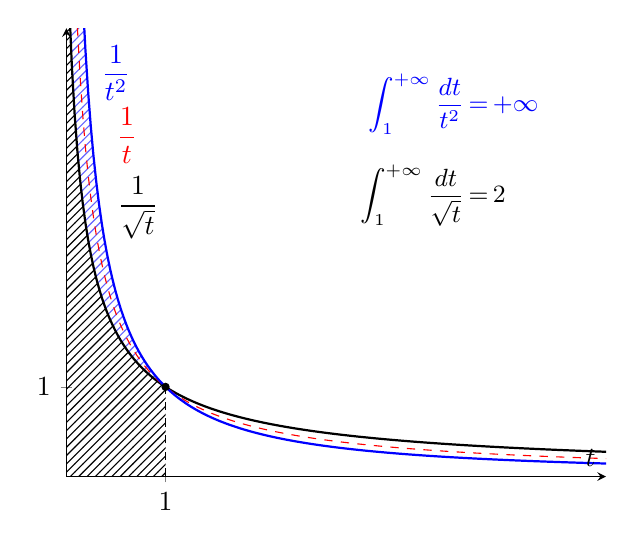
\begin{tikzpicture}
\begin{axis}[
    xmin=0.1, xmax=5,
    ymin=0, ymax=5,
    axis lines=middle,
    xlabel={$t$},
    domain=0.1:5,
    samples=200,
    thick,
    xtick={1},
    ytick={1},
]

% Aire hachurée sous 1/\sqrt{t} entre 0 et 1 (noir)
\addplot[domain=0:1, samples=100, pattern=north east lines,
         pattern color=black, draw=none, forget plot] {1/x^0.8} \closedcycle;

% Courbes nommées pour la zone entre les deux
\addplot[name path=A, draw=none, domain=0:1, samples=100, forget plot] {1/x^0.8};
\addplot[name path=B, draw=none, domain=0:1, samples=100, forget plot] {1/x^1.2};


% Aire hachurée entre 1/t et 1/t^2 (bleu, même sens que le noir)
\addplot[pattern=north east lines, pattern color=blue!60, forget plot]
    fill between[of=A and B];

% Courbe de t -> 1/\sqrt{t}
\addplot[black, thick] {1/x^0.8};

% Courbe de t -> 1/t
\addplot[red, dashed] {1/x};

% Courbe de t -> 1/t^2
\addplot[blue, thick] {1/x^1.2};

% Etiquettes des courbes sur l'axe des y (à droite de l'axe)
\node[black] at (axis cs:0.75,3) {$\dfrac{1}{\sqrt{t}}$};
\node[red] at (axis cs:0.65,3.8) {$\dfrac{1}{t}$};
\node[blue] at (axis cs:0.55,4.5) {$\dfrac{1}{t^2}$};

% Trait pointillé en x=1
\draw[dashed] (axis cs:1,0) -- (axis cs:1,1);

% Point d'intersection des deux courbes en (1,1)
\fill[black] (axis cs:1,1) circle (1.5pt);

% Résultats des intégrales, alignés, en haut à droite (légèrement décalés)
\node[anchor=north east, font=\small] at (axis cs:4.6,4.6) {
$\begin{array}{r@{\,}c@{\,}l}
\textcolor{blue}{\displaystyle\int_{1}^{+\infty}\dfrac{dt}{t^2}} & \textcolor{blue}{=} & \textcolor{blue}{+\infty}\\[16pt]
    \displaystyle\int_{1}^{+\infty}\dfrac{dt}{\sqrt{t}} & \textcolor{black}{=} & \textcolor{black}{2}
\end{array}$
};

\end{axis}
\end{tikzpicture}
\end{document}
